\begin{name}
{\tenchude}{\tendethi}{LỚP TOÁN THẦY PHÁT}{\thoigian}
\end{name}

\Opensolutionfile{ans}[ans/ansBTTeX1]
\begin{ex}%[2D3Y1-1]%
Xét $f(x), g(x)$ là các hàm số có đạo hàm liên tục trên $\mathbb{R}$. Phát biểu nào sau đây sai?
\choice
{$\displaystyle\int\limits(f(x)+g(x))\mathrm{d}x=\displaystyle\int\limits f(x)\mathrm{d}x+\displaystyle\int\limits g(x)\mathrm{d}x$}
{$\displaystyle\int\limits(f(x)-g(x))\mathrm{d}x=\displaystyle\int\limits f(x)\mathrm{d}x-\displaystyle\int\limits g(x)\mathrm{d}x$}
{\True $\displaystyle\int\limits(f(x))^2\mathrm{d}x=\left(\displaystyle\int\limits f(x)\mathrm{d}x\right)^2$}
{$\displaystyle\int\limits f(x)\mathrm{d}(g(x))=f(x).g(x)-\displaystyle\int\limits g(x)\mathrm{d}(f(x))$}
\loigiai{}
\end{ex}

\begin{ex}Câu 15%[2D3Y1-1]%
Họ tất cả các nguyên hàm của hàm số $f(x)=2x+5$ là
\choice
{\True $x^2+5x+C$}
{$2x^2+5x+C$}
{$Oz$}
{$x^2+C$}
.
\loigiai{
Ta có $\displaystyle\int (2x+5)\mathrm{\,d}x=x^2+5x+C$.}
\end{ex}

\begin{ex}%[2D3B1-1]%
Họ các nguyên hàm $\displaystyle\int \dfrac{1}{\sqrt{x}} \mathrm{\,d}x$ bằng
\choice
{$\dfrac{1}{\sqrt{x}}+C$}
{$\sqrt{x}+C$}
{$\dfrac{2}{\sqrt{x}}+C$}
{\True $2\sqrt{x}+C$}
\loigiai{
$\displaystyle\int \dfrac{1}{\sqrt{x}} \mathrm{\,d}x=\displaystyle\int x^{-\frac{1}{2}} \mathrm{\,d}x=\dfrac{x^{\frac{1}{2}}}{\dfrac{1}{2}}+C=2\sqrt{x}+C$.}
\end{ex}

\begin{ex}%[2D3B1-1]%Câu 9
Cho hàm số $f(x)=x^2+1$. Khẳng định nào dưới đây đúng?
\choice
{$\displaystyle\int{f(x){\rm{\,d}}x}=x^3+x+C$}
{\True $\displaystyle\int{f(x){\rm{\,d}}x}=\dfrac{x^3}{3}+x+C$}
{$\displaystyle\int{f(x){\rm{\,d}}x}=x^2+x+C$}
{$\displaystyle\int{f(x){\rm{\,d}}x}=2x+C$}
\loigiai{
Ta có $\displaystyle\int{f(x){\rm{\,d}}x}=\displaystyle\int{(x^2+1){\rm{\,d}}x}=\dfrac{x^3}{3}+x+C$.
}
\end{ex}

\begin{ex}%[2D3B1-2]%
Họ nguyên hàm $F(x)=\displaystyle \int\dfrac{\cos x}{4-\sin^2x}\mathrm{\,d}x$ tương ứng là
\choice
{$F(x)=\dfrac{1}{4}\ln \dfrac{2-\sin x}{2+\sin x}+C$}
{\True $F(x)=\dfrac{1}{4}\ln \dfrac{2+\sin x}{2-\sin x}+C$}
{$F(x)=\dfrac{1}{2}\ln \dfrac{2+\sin x}{2-\sin x}+C$}	{$F(x)=\dfrac{1}{2}\ln \dfrac{2-\sin x}{2+\sin x}+C$}
\loigiai{
Ta có: Đặt $t=\sin x \Rightarrow \mathrm{\,d}t=\cos x\mathrm{\,d}x $.\\
Suy ra $\displaystyle \int\dfrac{\cos x}{4-\sin^2x}\mathrm{\,d}x=\displaystyle \int\dfrac{1}{4-t^2}\mathrm{\,d}t=\displaystyle \int\dfrac{1}{(2-t)(2+t)}\mathrm{\,d}t=\dfrac{1}{4}\ln \dfrac{2+t}{2-t}+C=\dfrac{1}{4}\ln \dfrac{2+\sin x}{2-\sin x}+C$.
}
\end{ex}

\begin{ex}%[2D3B1-3]%
Họ nguyên hàm $F(x)=\displaystyle\int\mathrm{e}^{\sqrt{x}}\mathrm{\,d}x$ là
\choice
{$F(x)=\dfrac{1}{2\sqrt{x}}\mathrm{e}^{\sqrt{x}}+C$}
{\True $F(x)=2\mathrm{e}^{\sqrt{x}}\left(\sqrt{x}-1\right)+C$}
{$F(x)=\mathrm{e}^{\tfrac{2}{3}x\sqrt{x}}+C$}
{$F(x)=\mathrm{e}^{\sqrt{x}}\left(\sqrt{x}+2\right)+C$}
\loigiai{
Đặt $\sqrt{x}=t \Rightarrow x=t^2 \Rightarrow \mathrm{\,d}x=2t\mathrm{\,d}t$.\\
Suy ra $F(x)=\displaystyle\int\mathrm{e}^{\sqrt{x}}\mathrm{\,d}x=2\displaystyle\int\mathrm{e}^{t}\mathrm{\,d}t$.\\
Đặt $\heva{&u=t\\&\mathrm{e}^{t}\mathrm{\,d}t=\mathrm{\,d}v} \Rightarrow \heva{&\mathrm{\,d}u=\mathrm{\,d}t\\&v=\mathrm{e}^{t}.}$\\
Khi đó $F(x)=2t\cdot\mathrm{e}^{t}-2\displaystyle\int\mathrm{e}^{t}\mathrm{\,d}t=2t\cdot\mathrm{e}^{t}-2\mathrm{e}^{t}+C=2\mathrm{e}^{\sqrt{x}}\left(\sqrt{x}-1\right)+C$.
}
\end{ex}

\begin{ex}Câu 35%[2D3Y2-1]%
Biết $\displaystyle\int\limits_1^3 f(x)\mathrm{\,d}x=4$. Giá trị của $\displaystyle\int\limits_1^3 [5f(x)-1]\mathrm{\,d}x$ bằng
\choice
{$-22$}
{$22$}
{\True $18$}
{$20$}
\loigiai{
Xét $\displaystyle\int\limits_1^3 [5f(x)-1]\mathrm{\,d}x=5\displaystyle\int\limits_1^3 f(x)\mathrm{\,d}x-\displaystyle\int\limits_1^3 1\mathrm{\,d}x=18$.
}
\end{ex}

\begin{ex}%[2D3Y2-1]% Cau 23
Nếu $\displaystyle\int\limits_0^2 \dfrac{f\left( x \right)}{3} \mathrm{\,d}x=4$ thì$\displaystyle\int\limits_0^2 f\left( x \right)\mathrm{\,d}x $ bằng:
\choice
{\True $12$}
{ $4$}
{ $3^4$}
{ $\dfrac{4}{3}$}
\loigiai{
Do $\displaystyle\int\limits_0^2 \dfrac{f\left( x \right)}{3} \mathrm{\,d}x=4\Leftrightarrow \dfrac{1}{3}\displaystyle\int\limits_0^2 f\left( x \right) \mathrm{\,d}x=4\Leftrightarrow \displaystyle\int\limits_0^2 f\left( x \right) \mathrm{\,d}x=12$.}
\end{ex}

\begin{ex}Câu 35%[2D3B2-1]%
\immini[thm]
{Hình phẳng $S$ gồm hai phần được đánh dấu trong hình vẽ bên. Diện tích hình $S$ được tính theo công thức nào dưới đây?
\choice
{$S=-\displaystyle\int\limits_{-2}^0f(x)\mathrm{d}x-\displaystyle\int\limits_0^3f(x)\mathrm{d}x$}
{$S=\displaystyle\int\limits_{-2}^0f(x)\mathrm{d}x-\displaystyle\int\limits_0^3f(x)\mathrm{d}x$}
{$S=\displaystyle\int\limits_{-2}^0f(x)\mathrm{d}x+\displaystyle\int\limits_0^3f(x)\mathrm{d}x$}
{\True $S=-\displaystyle\int\limits_{-2}^0f(x)\mathrm{d}x+\displaystyle\int\limits_0^3f(x)\mathrm{d}x$}}
{\begin{tikzpicture}
\def\hsf(#1){0.02*(#1)^4-0.31*(#1)^3+0.17*(#1)^2+1.67*(#1)}
\def\hsg(#1){0}
\path[name path=dtf] plot[domain=-2.42:3.49] (\x,{\hsf(\x)});
\path[name path=dtg] plot[domain=-2.42:3.49]
(\x,{\hsg(\x)});
\path[name intersections={of=dtf and dtg,by={A,B,C}}];
\begin{scope}
\clip ($(A)+(90:2.2)$) rectangle ($(C)+(-90:2)$);
\fill[pattern=north east lines] plot[domain=-2.1:3.2] (\x,{\hsg(\x)})--plot[domain=3.2:-2.1] (\x,{\hsf(\x)})
;
\end{scope};
\draw[-stealth] (-2.3,0)--(3.4,0)node[below]{$x$};
\draw[-stealth] (0,-2.2)--(0,3)node[left]{$y$};
\draw[samples=100,domain=-2.2:3.2] plot (\x,{\hsf(\x)});
\path (0,0)node[above left]{$O$}
(A)node[above right]{$-2$}
(C)node[below left]{$3$}
;
\end{tikzpicture}}
\loigiai{
Dựa vào hình vẽ ta có $S=\displaystyle\int\limits_{-2}^0\left| f(x)\right|\mathrm{d}x+\displaystyle\int\limits_0^3\left| f(x)\right|\mathrm{d}x$ $=-\displaystyle\int\limits_{-2}^0f(x)\mathrm{d}x+\displaystyle\int\limits_0^3f(x)\mathrm{d}x$
}
\end{ex}

\begin{ex}%[Dự án Tex hóa Tư Duy Mở]%[Nhật Thiện]%[2D3B2-2]%
Cho tích phân $I=\displaystyle\int\limits_0^{\frac{\pi}{4}} \dfrac{1+\sin^2x}{2+\cos^2x} \mathrm{\,d}x$, nếu ta dùng một phép đổi biến số đặt $t=\tan x$ thì sẽ thu được tích phân tương ứng là
\choice
{$I=\displaystyle\int\limits_0^1 \dfrac{(2t^1+1)\mathrm{\,d}t}{2t^3+3}\mathrm{\,d}t$}
{$I=\displaystyle\int\limits_0^1 \dfrac{(2t^2+2)\mathrm{\,d}t}{(2t^2+3)(t^2+3)}$}
{$I=\displaystyle\int\limits_0^1 \dfrac{(2t^2+1)(t^2+1)\mathrm{\,d}t}{2t^2+3}$}
{\True $I=\displaystyle\int\limits_0^1 \dfrac{(2t^2+1)\mathrm{\,d}t}{(2t^2+3)(t^2+1)}$}
\loigiai{
Đặt $t=\tan x\Rightarrow \mathrm{\,d}t=(1+\tan^2 x) \mathrm{\,d}x\Rightarrow \dfrac{\mathrm{\,d}t}{(1+t^2)}=\mathrm{\,d}x$. Đổi cận $\heva{&x=0\Rightarrow t=0\\&x=\dfrac{\pi}{4}\Rightarrow t=1.}$\\
Ta có
\allowdisplaybreaks
\begin{eqnarray*}
I&=&\displaystyle\int\limits_0^{\frac{\pi}{4}} \dfrac{1+\sin^2x}{2+\cos^2x} \mathrm{\,d}x =\displaystyle\int\limits_0^{\frac{\pi}{4}} \left[\dfrac{\dfrac{1}{\cos^2x}+\tan^2x}{\dfrac{2}{\cos^2x}+1}\right] \mathrm{\,d}x=\dfrac{1}{2}\displaystyle\int\limits_0^{\frac{\pi}{4}} \left[\dfrac{1+2\tan^2x}{2\tan^2x+3}\right]\mathrm{\,d}x\\
&=&\dfrac{1}{2}\displaystyle\int\limits_0^{\frac{\pi}{4}} \left[\dfrac{1+2t^2}{2t^2+3}\right]\dfrac{\mathrm{\,d}t}{1+t^2}=\displaystyle\int\limits_0^1 \dfrac{(2t^2+1)\mathrm{\,d}t}{(2t^2+3)(t^2+1)}.
\end{eqnarray*}
}
\end{ex}

\begin{ex}%[2D3B2-2]%Câu 458.
Tích phân $I=\displaystyle\int_0^\pi\cos ^3 x\sin x \mathrm{\,d}x$ bằng
\choice
{$-\dfrac{1}{4}\pi^4$}
{$-\dfrac{1}{4}$}
{\True $0$}
{$-\pi^4$}
\loigiai{
Đặt $u=\cos x\Rightarrow \mathrm{\,d}u=-\sin x\mathrm{\,d}x$.\\
Đổi cận: $x=0\Rightarrow u=1$; $x=\pi\Rightarrow u=-1$.\\
Suy ra $I=\displaystyle\int_{-1}^1 u^3 \mathrm{\,d}u=\dfrac{1}{4}u^4\bigg|_{-1}^1=0$.
}
\end{ex}

\begin{ex}%[2D3B2-3]%
Cho $f(x)$ có đạo hàm trên $[1; 2]$ thỏa $\heva{&f(1)=0 \\ &f(2)=2}$ và $\displaystyle\int\limits_1^2 f(x)\mathrm{\,d}x=1$,  khi đó $\displaystyle\int\limits_1^2 x\cdot f'(x)\mathrm{\,d}x $ bằng
\choice
{$2$}
{$\dfrac{1}{2}$}
{$\dfrac{8}{3}$}
{\True $3$}
\loigiai{
Đặt $\heva{&u=x\Rightarrow \mathrm{\,d}u=\mathrm{\,d}x\\&\mathrm{\,d}v=f'(x) \mathrm{\,d}x\Rightarrow v=f(x).}$\\
Suy ra $\displaystyle\int\limits_1^2 xf'(x) \mathrm{\,d}x=x\cdot f(x) \Big|_1^2 -\displaystyle\int\limits_1^2 f(x) \mathrm{\,d}x=2f(2)-f(1)-1=3$.
}
\end{ex}

\begin{ex}%[2D3B2-3]%Câu 470.
Biết $\displaystyle\int_0^1(2 x+1) \mathrm{e}^x \mathrm{\,d}x=a+ b\mathrm{e}$ với $a$, $b\in \mathbb{R}$. Giá trị của biểu thức $a^3+b$ bằng
\choice
{$25$}
{\True $2$}
{$9$}
{$17$}
\loigiai{
Đặt $\heva{& u=2x+1\Rightarrow \mathrm{\,d}u=2\mathrm{\,d}x \\ & \mathrm{\,d}v=\mathrm{e}^x \mathrm{\,d}x\Rightarrow v=\mathrm{e}^x.}$\\
Khi đó $\displaystyle\int_0^1(2 x+1) \mathrm{e}^x \mathrm{\,d}x=(2x+1)\mathrm{e}^x\bigg|_0^1-\displaystyle\int_0^1 2\mathrm{e}^x \mathrm{\,d}x=3\mathrm{e}-1-2\mathrm{e}^x\bigg|_0^1=\mathrm{e}+1$.\\
Vậy $a^3+b=1^3+1=2$.
}
\end{ex}

\begin{ex}%[2D3Y3-3]%
Thể tích khối tròn xoay sinh ra khi quay hình phẳng giới hạn bởi đồ thị các hàm số $y=x^2-2x$, $y=0$, $x=-1$, $x=2$ quanh trục $Ox$ bằng
\choice
{$\dfrac{16\pi}{5}$}
{$\dfrac{17\pi}{5}$}
{\True $\dfrac{18\pi}{5}$}
{$\dfrac{5\pi}{18}$}
\loigiai{
Thể tích của khối tròn xoay đã cho bằng
$$V=\pi\displaystyle\int\limits_{-1}^{2}\left(x^2-2x\right)^2\mathrm{\,d}x=\pi\displaystyle\int\limits_{-1}^{2}\left(x^4-4x^3+4x^2\right)\mathrm{\,d}x=\pi\left(\dfrac{x^5}{5}-x^4+\dfrac{4}{3}x^3\right)\biggr|_{-1}^{2}=\dfrac{18\pi}{5}.$$
}
\end{ex}

\begin{ex}%[2D3Y3-1]%Câu 484.
Diện tích $S$ của hình phẳng giói hạn bởi các đường $y=2x^2$, $y=-1$, $x=0$ và $x=1$ được tính bởi công thức nào sau đây?
\choice
{$S=\pi\displaystyle\int_0^1(2x^2+1) \mathrm{\,d}x$}
{$S=\displaystyle\int_0^1(2x^2-1) \mathrm{\,d}x$}
{$S=\displaystyle\int_0^1(2x^2+1)^2 \mathrm{\,d}x$}
{\True $S=\displaystyle\int_0^1(2x^2+1) \mathrm{\,d}x$}
\loigiai{
Xét $f_1(x)-f_2(x)=2x^2-(-1)=2x^2+1>0,\forall x$.\\
Do đó diện tích $S=\displaystyle\int_0^1(2x^2+1) \mathrm{\,d}x$.
}
\end{ex}

\begin{ex}%[2D3Y3-1]%  Câu 35:
Diện tích hình phẳng được gạch chéo trong dưới đây bằng
\begin{center}
\begin{tikzpicture}
\def\xmin{-2.1}
\def\xmax{2.1}
\def\xminb{-1.5}
\def\xmaxb{2.5}
\def\hsf(#1){0.5*(#1)^4-(#1)^2-2.5}
\def\hsg(#1){1.5*(#1)-1.5}
\draw[->](-2.5,0)--(4,0);
\draw[->](0,-3.4)--(0,3.5);
\draw (4,0) node[above]{$x$} (0,3.5) node[left]{$y$} (0,0) node[below right]{$O$};
\draw[smooth,color=blue] plot[domain=\xmin:\xmax] (\x,{\hsf(\x)}) node[above]{$y=\dfrac{1}{2}x^4-x^2-\dfrac{5}{2}$};
\draw[smooth,color=red] plot[domain=\xminb:\xmaxb] (\x,{\hsg(\x)}) node[below right]{$y=\dfrac{3}{2}x-\dfrac{3}{2}$};
\path[name path=dtf] plot[domain=\xmin:\xmax] (\x,{\hsf(\x)});
\path[name path=dtg] plot[domain=\xminb:\xmaxb]
(\x,{\hsg(\x)});
\path[name intersections={of=dtf and dtg,by={A,B}}];
\begin{scope}
%\clip ($(A)+(90:2.2)$) rectangle ($(B)+(-90:2)$);
%\clip ($(A)$) rectangle ($(B))$);
\fill[pattern=north east lines] plot[domain=-1:2] (\x,{\hsg(\x)})--plot[domain=2:-1] (\x,{\hsf(\x)})
;
\end{scope};
\draw(-1,0) circle (.03) node[below left]{$-1$};
\draw(2,0) circle (.03) node[below right]{$2$};
\draw(0,-3) circle (.03) node[below right]{$-3$};
\draw(0,1.5) circle (.03) node[above right]{$\dfrac{3}{2}$};
\draw [dashed] (-1,0)--(-1,-3)--(0,-3);
\draw [dashed] (2,0)--(2,1.5)--(0,1.5);
\end{tikzpicture}

\end{center}
\choice
{$\int\limits_{-1}^2{\left(\dfrac{1}{2}x^4-x^2-\dfrac{3}{2}x-1\right)\mathrm{\,d}x}$}
{$\int\limits_{-1}^2{\left(-\dfrac{1}{2}x^4+x^2+\dfrac{3}{2}x+4\right)\mathrm{\,d}x}$}
{$\int\limits_{ - 1}^2 {\left( { - \frac{1}{2}{x^4} - {x^2} - \frac{3}{2}x - 4} \right)} \mathrm{\,d}x$}
{\True $\int\limits_{-1}^2{\left(-\dfrac{1}{2}x^4+x^2+\dfrac{3}{2}x+1\right)}\mathrm{\,d}x$}
\loigiai{
Diện tích hình phẳng được gạch chéo trong hình bên bằng:\\
$\int\limits_{-1}^2{\left(\dfrac{3}{2}x-\dfrac{3}{2}-\dfrac{1}{2}x^4+x^2+\dfrac{5}{2}\right)}\mathrm{\,d}x$ $=\int\limits_{-1}^2{\left(-\dfrac{1}{2}x^4+x^2+\dfrac{3}{2}x+1\right)}\mathrm{\,d}x$.}
\end{ex}

\begin{ex}%[2D3B3-1]%Câu 30
Diện tích $S$ của hình phẳng giới hạn bởi đồ thị hàm số $y=x^2$ và $y=x+2$ được tính theo công thức
\choice
{$S=\displaystyle\int\limits_{-1}^2\left(x^2-x-2\right)\mathrm{\,d}x$}
{\True $S=\displaystyle\int\limits_{-1}^2\left(-x^2+x+2\right)\mathrm{\,d}x$}
{$S=\pi\displaystyle\int\limits_{-1}^2\left(x^2-x-2\right)\mathrm{\,d}x $}
{$S=\pi\displaystyle\int\limits_{-1}^2\left(-x^2+x+2\right)\mathrm{\,d}x$}
\loigiai{
Ta có $x^2=x+2\Leftrightarrow x^2-x-2=0\Leftrightarrow\hoac{& x=-1\\
& x=2.}$\\
Suy ra $ S=\displaystyle\int\limits_{-1}^2\left| x^2-x-2\right|\mathrm{\,d}x  $ mà $x^2-x-2<0,\, \forall x\in\left(-1;2\right)$ nên $S=\displaystyle\int\limits_{-1}^2\left(-x^2+x+2\right)\mathrm{\,d}x $ .}
\end{ex}

\begin{ex}%[2D3B3-3]%
Thể tích của khối tròn xoay khi quay hình phẳng giới hạn bởi đồ thị hàm số $y=x^2-x$ và trục hoành quanh trục hoành là
\choice
{$\dfrac{\pi}{3}$}
{\True $\dfrac{\pi}{30}$}
{$\dfrac{\pi}{15}$}
{$\dfrac{\pi}{5}$}
\loigiai{
Phương trình hoành độ giao điểm của đồ thị hàm số $y=x^2-x$ và trục hoành là\\
$x^2-x=0\Leftrightarrow\hoac{&x=0\\&x=1.}$ \\
Vậy $V=\pi\displaystyle\int\limits_0^1\left(x^2-x\right)^2\mathrm{\,d}x=\dfrac{\pi}{30}$.}
\end{ex}

\begin{ex}%[2D4Y1-1]%
Số phức liên hợp của $3+i$ bằng
\choice
{\True $3-i$}
{$i-3$}
{$-3-i$}
{$3i$}
\loigiai{
Số phức liên hợp của $3+i$ là $3-i$.
}
\end{ex}

\begin{ex}%[2D4Y1-1]%
Cho số phức $z=1-2 i$. Tìm phần ảo của số phức $\bar{z}$.
\choice
{\True $2$}
{$-2$}
{$-1$}
{$1$}
\loigiai{
Ta có $z=1-2 i \Rightarrow \bar{z}=1+2 i$.\\
Vậy $\bar{z}$ có phần ảo $b=2$.
}
\end{ex}

\begin{ex}%[2D4Y1-2]%
Trong mặt phẳng $Oxy$, số phức $z=-2+4i$ được biểu diễn bởi điểm nào trong các điểm ở hình vẽ dưới đây?
\begin{center}
\begin{tikzpicture}[scale=0.7, font=\footnotesize, line join=round, line cap=round,>=stealth]
\def\xmin{-5} \def\xmax{5}
\def\ymin{-5} \def\ymax{5}
\draw[->] (\xmin,0)--(\xmax,0) node [below]{$x$};
\draw[->] (0,\ymin)--(0,\ymax) node [left]{$y$};
\node at (0,0) [below left]{$O$};
\clip (\xmin+0.1,\ymin+0.1) rectangle (\xmax-0.1,\ymax-0.1);
\draw[dashed] (0,-4)node[left]{$-4$}--(2,-4)--(2,0)node[above]{$2$}
(-4,0)node[below]{$-4$}--(-4,2)--(0,2)node[right]{$2$}
(-2,0)node[below]{$-2$}--(-2,4)--(0,4)node[right]{$4$}
(0,-2)node[left]{$-2$}--(4,-2)--(4,0)node[above]{$4$}
;
\fill (2,-4)node[right]{$B$} circle (1.0pt) (-4,2)node[left]{$A$} circle (1.0pt)
(-2,4)node[left]{$C$} circle (1.0pt) (4,-2)node[right]{$D$} circle (1.0pt);
\end{tikzpicture}
\end{center}
\choice
{\True Điểm $C$}
{Điểm $D$}
{Điểm $A$}
{Điểm $B$}
\loigiai{
Số phức $z=-2+4i$ có điểm biểu diễn là điểm $C(-2;4)$.}
\end{ex}

\begin{ex}%[2D4Y1-2]%
Số phức $ z=a+bi\,(a, b\in\mathbb{R}) $  có điểm biểu diễn như hình vẽ bên dưới. Tìm $ a $  và  $ b $.
\begin{center}
\begin{tikzpicture}[line cap=butt,line join=miter,>=stealth]
\tikzset{declare function={xmin=-2;xmax=4;ymin=-4.5;ymax=1;},
smooth,samples=450
}
\draw[->] (xmin,0)--(xmax,0) node[shift={(-100:7pt)},font=\normalsize]{$ x $};
\draw[->] (0,ymin)--(0,ymax) node[shift={(190:7pt)},font=\normalsize]{$ y $};
\fill (0,0) node[shift={(225:7pt)},font=\normalsize]{$ O $};
\clip (xmin,ymin) rectangle (xmax,ymax);
\draw[dashed] (3,0)node[above]{$ 3 $}--(3,-4)node[below]{$ M $}--(0,-4)node[left]{$ -4 $};
\end{tikzpicture}
\end{center}
\choice
{$ a=-4 $, $ b=3 $}
{$ a=3 $, $ b=4 $}
{\True $ a=3 $, $ b=-4 $}
{$ a=-4 $, $ b=-3 $}
\loigiai{
Ta có 	$ a=3 $, $ b=-4 $.
}
\end{ex}

\begin{ex}%[2D4B1-1]%Câu 18
Cho số phức $ z=a+bi\left(a,b\in\mathbb{R}\right)$ thỏa mãn $z-2\bar{z}=-1+6i$. Giá trị $a+b$ bằng
\choice
{\True $3$}
{$-3$}
{$2$}
{$-1$}
\loigiai{
Ta có\\
$ z-2\bar{z}=-1+6i\Leftrightarrow a+bi-2\left(a-bi\right)=-1+6i\Leftrightarrow-a+3bi=-1+6i\Leftrightarrow\left\{\begin{aligned}
&-a=-1\\
& 3b=6\\
\end{aligned}\right.\Leftrightarrow\left\{\begin{aligned}
& a=1\\
& b=2.\\
\end{aligned}\right.$\\
Vậy $ a+b=1+2=3$.}
\end{ex}

\begin{ex}%[2D4B1-2]% ::Cau 7::

Điểm biểu diễn của số phức $z$ là $M\left( 1\,;2 \right)$. Toạ độ của điểm biểu diễn số phức $w=z-2\bar{z}$ là
\choice
{ $\left( 2\,;3 \right)$}
{ $\left( 2\,;1 \right)$}
{\True $\left( -1\,;6 \right)$}
{ $\left( 2\,;-3 \right)$}
\loigiai{
Ta có $z=1+2i \Rightarrow \bar{z}=1-2i$.\\
$w=\left( 1+2i \right)-2\left( 1-2i \right)\Leftrightarrow w=-1+6i$.\\
Vậy điểm biểu diễn của số phức $w$ là $\left( -1\,;6 \right)$.}
\end{ex}

\begin{ex}%[Vanle Vo]%[2D4Y2-1]%Câu 19
Cho số phức $z_1=1-2i$; $z_2=3+4i$. Tìm phần ảo của số phức $w=2z_1+3z_2$.
\choice
{$3$}
{$6$}
{\True $8$}
{$5$}
\loigiai{
$w=2z_1+3z_2=11+8i$. Phần ảo bằng $8$.
}
\end{ex}

\begin{ex}%[2D4Y2-2]% Cau 15
Cho số phức $z$ thỏa mãn $\left( 1-2i \right)z=-2-11i$. Tính số phức liên hợp của số phức $z$.
\choice
{\True $\bar{z}=4+3i$}
{ $\bar{z}=4-3i$}
{ $\bar{z}=-4-3i$}
{ $\bar{z}=-4+3i$}
\loigiai{
Ta có $z=\dfrac{-2-11i}{1-2i}=4-3i$.\\
Nên $\bar{z}=4+3i$.}
\end{ex}

\begin{ex}%[2D4B2-1]% ::Cau 21::

Cho số phức $z=2+3i$. Tìm số phức $w=\left( 3+2i \right)z+2\bar{z}$.
\choice
{\True $w=4+7i$}
{ $w=5+7i$}
{ $w=7+4i$}
{ $w=7+5i$}
\loigiai{
Ta có $w=\left( 3+2i \right)z+2\bar{z}=\left( 3+2i \right)\left( 2+3i \right)+2\left( 2-3i \right)$ $=13i+4-6i=4+7i$.\\
Vậy $w=4+7i$.}
\end{ex}

\begin{ex}Câu 35%[2D4Y3-1]%
Cho số phức $z$ thỏa mãn $iz=5+4i$. Số phức liên hợp của $z$ là
\choice
{\True $\overline{z}=4+5i$}
{$\overline{z}=4-5i$}
{$\overline{z}=-4+5i$}
{$\overline{z}=-4-5i$}
\loigiai{
Ta có $iz=5+4i$ $\Rightarrow z=\dfrac{5+4i}{i} \Rightarrow z=4-5i$ $\Rightarrow \overline{z}=4+5i$.
}
\end{ex}

\begin{ex}%[2D4B3-2]%
Môđun của số phức $\omega=z+z^2$, với $z$ là số phức thỏa mãn $(2+i) z+\dfrac{1-i}{1+i}=5-i$ là.
\choice
{$2 \sqrt{2}$}
{$4 \sqrt{2}$}
{\True $5 \sqrt{2}$}
{$3 \sqrt{2}$}
\loigiai{
$(2+i) z+\dfrac{1-i}{1+i}=5-i \Leftrightarrow z=2-i \Rightarrow z^2=3-4i$.
$\Rightarrow \omega=5-5i \Rightarrow|\omega|=5 \sqrt{2}$.
}
\end{ex}

\begin{ex}%[2D4B3-2]%
Cho số phức $z$ thỏa mãn phương trình $(2-3i)z=5+11i$. Phần thực của số phức $z$ bằng
\choice
{\True $-\dfrac{23}{13}$}
{$\dfrac{37}{13}$}
{$\dfrac{23}{13}$}
{$-\dfrac{23}{146}$}
\loigiai{
Ta có $(2-3i)z=5+11i \Leftrightarrow z=\dfrac{5+11i}{2-3i}=-\dfrac{23}{13}+\dfrac{37}{13}i$.\\
Phần thực của số phức $z$ bằng $-\dfrac{23}{13}$.
}
\end{ex}

\begin{ex}%[Vũ Ngọc Phát]%[TDM]%[2D4B3-4]%
Cho số phức $z$ thỏa mãn $|(1+2i)z-5|=|(2-i)z-10|$. Trên mặt phẳng tọa độ $Oxy$ tập hợp điểm biểu diễn số phức $z$ là
\choice
{đường thẳng $3x-4y-7=0$}
{đường thẳng $2x+y-1=0$}
{\True đường thẳng $6x-8y-13=0$}
{đường thẳng $6x+8y-15=0$}
\loigiai{
Gọi $z=x+yi$, $x$, $y\in \mathbb{R}$.
\begin{eqnarray*}
&&\left| (1+2i)z-5 \right|=\left| (2-i)z-10 \right| \\
&\Leftrightarrow& |1+2i||z-1+2i|=|2-i||z-4-2i| \\
&\Leftrightarrow& \sqrt{5}\left[(x-1)^2+(y+2)^2\right] = \sqrt{5}\left[(x-4)^2+(y-2)^2\right] \\
&\Leftrightarrow& 6x+8y-13=0.
\end{eqnarray*}
}
\end{ex}

\begin{ex}%[2D4B4-1]%[Câu 18]%
Gọi $z_1$, $z_2$ là các nghiệm phức của phương trình $2z^2-2z+5=0$ với phần ảo lần lượt là dương và âm. Số phức liên hợp của số phức $w=4-z_1^2+z_2^2$ là
\choice
{$\overline{w}=4-3i$}
{\True $\overline{w}=4+3i$}
{$\overline{w}=-4+3i$}
{$\overline{w}=-4-3i$}
\loigiai{
Ta có $2z^2-2z+5=0$ $\Leftrightarrow \hoac{&z_1=\dfrac{1}{2}+\dfrac{3}{2}i \\&z_2=\dfrac{1}{2}-\dfrac{3}{2}i.}$\\
Theo giả thiết $w=4-z_1^2+z_2^2=4-\left(\dfrac{1}{2}+\dfrac{3}{2}i\right)^2+\left(\dfrac{1}{2}-\dfrac{3}{2}i\right)^2=4-3i\Rightarrow \overline{w}=4+3i$.}
\end{ex}

\begin{ex}%[Số phức - Tư duy mở]%[Hồng Trường Sơn]%[2D4Y4-1]%
Căn bậc hai của số phức $z=4$ là hai số phức
\choice
{\True $\pm 2$}
{$\pm 1$}
{$\pm 4$}
{$\pm 16$}
\loigiai{
Căn bậc hai của số phức $z=4$ là $\pm 2$.
}
\end{ex}

\begin{ex}Câu 15%[2H3Y1-1]%
Trong không gian $Oxyz$, cho hai điểm $A(2;-1;3)$, $B(3;2;-4)$. Véc-tơ $\overrightarrow{AB}$ có tọa độ là
\choice
{$(1;-3;-7)$}
{\True $(1;3;-7)$}
{$(-1;3;-7)$}
{$(-1;-3;-7)$}
\loigiai{
Ta có $\overrightarrow{AB}=(1;3;-7)$.
}
\end{ex}

\begin{ex}%[2H3B1-3]%
Trong không gian với hệ tọa độ $O x y z$, tìm tất cả các giá trị của tham số $m$ để phương trình $x^{2}+y^{2}+z^{2}-4 x+2 m y+6 z+13=0$ là phương trình của mặt cầu.
\choice
{$m>0$}
{\True $m \neq 0$}
{$m \in \mathbb{R}$}
{$m<0$}
\loigiai{
Để phương trình $x^{2}+y^{2}+z^{2}-4 x+2 m y+6 z+13=0$ là phương trình của mặt cầu thì $$4+m^{2}+3^{2}-13>0 \Leftrightarrow m^{2}>0 \Leftrightarrow m \neq 0.$$
}
\end{ex}

\begin{ex}%[2H3Y2-2]%Câu 15
Trong không gian $Oxyz$, cho mặt phẳng $(\alpha)\colon 3x+2y-4z+1=0$. Véc-tơ nào dưới đây là một véc-tơ pháp tuyến của $(\alpha)$?
\choice
{$\overrightarrow{n}_2=(3;2;4)$}
{$\overrightarrow{n}_3=(2;-4;1)$}
{$\overrightarrow{n}_1=(3;-4;1)$}
{\True $\overrightarrow{n}_4=(3;2;-4)$}
\loigiai{
Mặt phẳng $(\alpha)\colon 3x+2y-4z+1=0$ có một véc-tơ pháp tuyến là $\overrightarrow n=(3;2;-4)$.
}
\end{ex}

\begin{ex}Câu 10%[2H3Y2-4]%
Trong không gian $O x y z$, cho mặt phẳng $(P)\colon x-2 y+z-5=0$. Điểm nào dưới đây thuộc $(P)$ ?
\choice
{$Q(2 ;-1 ; 5)$}
{$P(0 ; 0 ;-5)$}
{ \True $M(1 ; 1 ; 6)$}
{$N(-5 ; 0 ; 0)$}
\loigiai{
Thay tọa độ các điểm $Q$, $P$, $M$, $N$ vào phương trình mặt phẳng $(P)$.
Ta thấy  với tọa độ của điểm $M$ thỏa mãn phương trình của $(P)$.\\ Vậy $M \in(P)$.}
\end{ex}

\begin{ex}%[2H3B2-3]%
Trong không gian $O x y z$, phương trình mặt phẳng đi qua ba điểm $A(1 ; 0 ; 2)$, $B(1 ; 1 ; 1)$, $C(2 ; 3 ; 0)$ là
\choice
{$x+y-z+1=0$}
{\True $x-y-z+1=0$}
{$x+y+z-3=0$}
{$x+y-2 z-3=0$}
\loigiai{
Ta có $\overrightarrow{AB}=(0;1;-1)$, $\overrightarrow{AC}=(1;3;-2)$.\\
Mặt phẳng đi qua điểm $A(1 ; 0 ; 2)$ và có véc-tơ pháp tuyến $\vec{n}=\left[\overrightarrow{AB},\overrightarrow{AC}\right]=(1;-1;-1)$ có phương trình là
$$1(x-1)-1(y-0)-1(z-2)=0\Leftrightarrow x-y-z+1=0.$$
}
\end{ex}

\begin{ex}%[DA TexBook 12, Họa Sĩ Sân Cỏ]%[2H3B2-3]%trùng câu 15
Trong không gian $Oxyz$, phương trình mặt phẳng $(P)$ đi qua điểm $B(2;1;-3)$, đồng thời vuông góc với hai mặt phẳng $(Q) \colon x+y+3z=0$, $(R) \colon 2x-y+z=0$?
\choice
{\True $4x+5y-3z-22=0$}
{$4x-5y-3z-12=0$}
{$2x+y-3z-14=0$}
{$4x+5y-3z+22=0$}
\loigiai{
$\vec{n}_{1}=(1;1;3)$ và $\vec{n}_{2}=(2;-1;1)$ lần lượt là các véc-tơ pháp tuyến của hai mặt phẳng $(Q)$ và $(R)$.\\
Vì mặt phẳng $(P)$ vuông góc với hai mặt phẳng $(Q)$ và $(R)$ nên ta chọn véc-tơ pháp tuyến mặt phẳng $(P)$ là $\vec{n}=\left[\vec{n}_{1},\vec{n}_{2}\right]=(4;5;-3)$.\\
Mà mặt phẳng $(P)$ đi qua điểm $B(2;1;-3)$ nên  phương trình mặt phẳng $(P)$ là $$4(x-2)+5(y-1)-3(z+3)=0 \Leftrightarrow 4x+5y-3z-22=0.$$
}
\end{ex}

\begin{ex}Câu 7%[2H3Y3-1]%
Trong không gian $Oxyz$, cho đường thẳng $d \colon \dfrac{x-2}{-1}=\dfrac{y-1}{2}=\dfrac{z+3}{1}$. Véc-tơ nào dưới đây là một véc-tơ chỉ phương của $d$?
\choice
{$\overrightarrow{u}_2=(2;1;1)$}
{$\overrightarrow{u}_4=(1;2;-3)$}
{\True $\overrightarrow{u}_3=(-1;2;1)$}
{$\overrightarrow{u}_1=(2;1;-3)$}
\loigiai{
Đường thẳng $d \colon \dfrac{x-2}{-1}=\dfrac{y-1}{2}=\dfrac{z+3}{1}$ có một véc-tơ chỉ phương là $\overrightarrow{u}_3=(-1;2;1)$.}
\end{ex}

\begin{ex}%[Hình học Oxyz, Tư duy mở]%[Lê Hồng Phi]%[2H3Y3-6]%
Trong không gian tọa độ $Oxyz$, cho hai đường thẳng $\Delta_1\colon \dfrac{x-1}{3}=\dfrac{y+2}{1}=\dfrac{z-1}{-2}$ và đường thẳng $\Delta_2\colon \dfrac{x+4}{4}=\dfrac{y-1}{-1}=\dfrac{z+5}{2}$. Nhận xét đúng về vị trí tương đối của hai đường thẳng $\Delta_1$, $\Delta_2$ là
\choice
{\True Hai đường thẳng cắt nhau tại $A(4;-1;-1)$}
{Hai đường thẳng cắt nhau tại $A(1;0;-3)$}
{Hai đường thẳng chéo nhau}
{Hai đường thẳng song song với nhau}
\loigiai{
Đường thẳng $\Delta_1$, $\Delta_2$ lần lượt có véc-tơ chỉ phương là $\overrightarrow{u}_1=(3;1;-2)$ và $\overrightarrow{u}_2=(4;-1;2)$.\\
Dễ thấy $\dfrac{3}{4}\neq\dfrac{1}{-1}$ nên $\Delta_1$ và $\Delta_2$ cắt nhau hoặc chéo nhau.\\
Phương trình tham số của $\Delta_1$ là $\Delta_1\colon\heva{& x=1+3t \\ & y=-2+t\\ & z=1-2t}, t\in\mathbb{R}$.\\
Phương trình tham số của $\Delta_2$ là $\Delta_2\colon\heva{& x=-4+4t' \\ & y=1-t'\\ & z=-5+2t'}, t'\in\mathbb{R}$.\\
Hệ phương trình $\heva{&  1+3t=-4+4t'\\ & -2+t=1-t'\\ & 1-2t=-5+2t'}\Leftrightarrow\heva{& t=1 \\ & t'=2.}$\\
Do đó $\Delta_1$ cắt $\Delta_2$ tại $A(4;-1;-1)$.
}
\end{ex}

\begin{ex}%[TexBook12-Quyen3, Biên soạn thầy Nguyễn Ngọc Nguyên - Phản biện thầy Nguyễn Sĩ Đạt]%[2H3Y3-3]%
Trong không gian với hệ tọa độ $Oxyz$. Đường thẳng $d \colon \heva{&x=t\\&y=1-t\\&z=2+t}$ đi qua điểm nào sau đây?
\choice
{$K(1;-1;1)$}
{$E(1;1;2)$}
{$H(1;2;0)$}
{\True $F(0;1;2)$}
\loigiai{
Thay tọa độ của $K(1;-1;1)$ vào PTTS của $d$ ta được
$\heva{&1=t\\&-1=1-t\\&1=2+t} \Leftrightarrow \heva{&t=1\\&t=2\\&t=-1}$. Không tồn tại $t$.\\
Do đó $K \notin d$.\\
Thay tọa độ của $E(1;1;2)$ vào PTTS của $d$ ta được
$\heva{&1=t\\&1=1-t\\&2=2+t} \Leftrightarrow \heva{&t=1\\&t=0\\&t=0}$. Không tồn tại $t$.\\
Do đó $E \notin d$.\\
Thay tọa độ của $H(1;2;0)$ vào PTTS của $d$ ta được
$\heva{&1=t\\&2=1-t\\&0=2+t} \Leftrightarrow \heva{&t=1\\&t=-1\\&t=-2}$. Không tồn tại $t$.\\
Do đó $H \notin d$.\\
Thay tọa độ của $F(0;1;2)$ vào PTTS của $d$ ta được
$\heva{&0=t\\&1=1-t\\&2=2+t} \Leftrightarrow \heva{&t=0\\&t=0\\&t=0} \Leftrightarrow t=0$.\\
Do đó $F \in d$.
}
\end{ex}

\begin{ex}%[2H3B3-2]%
Trong không gian $Oxyz$, viết phương trình đường thẳng $d$ đi qua điểm $M(1;2;3)$, đồng thời vuông góc với hai véc-tơ $\vec{a}=(2;3;0)$, $\vec{b}=(3;4;0)$.
\choice
{$\heva{& x=1+t \\ & y=2+t\\ &z=3+t}$}
{\True $\heva{& x=1 \\ & y=2\\ &z=3-t}$}
{$\heva{& x=t \\ & y=2\\ &z=3+t}$}
{$\heva{& x=1 \\ & y=t\\ &z=3}$}
\loigiai{
Gọi $\vec{u}$ là véc-tơ chỉ phương của đường thẳng $d$. Do đường thẳng $d$ vuông góc đồng thời với hai véc-tơ $\vec{a}=(2;3;0)$, $\vec{b}=(3;4;0)$ nên $\vec{u}=[\vec{a},\vec{b}]=(0;0;-1)$ làm véc-tơ chỉ phương và đi qua $M(1;2;3)$ nên có phương trình $\heva{& x=1 \\ & y=2\\ &z=3-t.}$
}
\end{ex}

\begin{ex}%[2H3B3-6]%
Trong không gian với hệ tọa độ $ Oxyz $, cho đường thẳng $d\colon \dfrac{x-1}{m}=\dfrac{y+2}{2 m-1}=\dfrac{z+3}{2}$ và mặt phẳng $(P)\colon  x+3 y-2 z+1=0$. Với giá trị nào của $m$ thì đường thẳng $d$ vuông góc mặt phẳng $ (P) $?
\choice
{$m=2$}
{\True $m=-1$}
{$m=1$}
{$m=0$}
\loigiai{
Yêu cầu bài toán tương đương $\overrightarrow{u}_{d}(m ; 2 m-1 ; 2)$ cùng phương $\overrightarrow{n}_{P}(1 ; 3 ;-2)$ hay $$\dfrac{m}{1}=\dfrac{2 m-1}{3}=\dfrac{2}{-2}=-1 \Rightarrow m=-1.$$
}
\end{ex}

\begin{ex}%[2D3K2-3]%
Giá trị của tích phân $I=\displaystyle \int\limits_{\frac{\pi}{6}}^{\frac{\pi}{3}} \cos x \ln\left(\sin x\right) \mathrm{d}x$ tương ứng bằng
\choice
{$\dfrac{\sqrt{3}}{2}-1$}
{\True $\dfrac{\sqrt{3}\ln 3 +\left(2-2\sqrt{3}\right)\left(\ln 2+1\right)}{4}$}
{$\dfrac{3\sqrt{3}-2}{4}$}
{$\sqrt{3}\ln3 -2\ln2+1$}
\loigiai{
Đây là tích phân từng phần. Đặt $\heva{
&u=\ln\left(\sin x\right) \\ & \mathrm{d}v =\cos x \mathrm{d}x} \Rightarrow \heva{
&\mathrm{d}u=\cos x \cdot \dfrac{\mathrm{d}x}{x}\\
&v = \sin x.}$\\
Suy ra $I=\displaystyle \int\limits_{\frac{\pi}{6}}^{\frac{\pi}{3}}\cos x \ln \left(\sin x\right)\mathrm{d}x=\sin x \ln \left(\sin x\right) \bigg|_{\frac{\pi}{6}}^{\frac{\pi}{3}} - \int\limits_{\frac{\pi}{6}}^{\frac{\pi}{3}}\sin x \cdot \cos x \dfrac{\mathrm{d}x}{\sin x}.$\\
Hay $I=\dfrac{\sqrt{3}}{2}\ln \dfrac{\sqrt{3}}{2}-\dfrac{1}{2}\ln\dfrac{1}{2} \displaystyle \int\limits_{\frac{\pi}{6}}^{\frac{\pi}{3}}\cos x \mathrm{d}x$.\\
Dẫn đến $I=\dfrac{\sqrt{3}}{2}\ln \dfrac{\sqrt{3}}{2}-\dfrac{1}{2}\ln\dfrac{1}{2}-\sin x \bigg|_{\frac{\pi}{6}}^{\frac{\pi}{3}}=\dfrac{\sqrt{3}\ln3+\left(2-2\sqrt{3}\right)\left(\ln 2+1\right)}{4}.$
}
\end{ex}

\begin{ex}%[2D3K2-2]%
Cho tích phân $I=\displaystyle\int\limits_{1}^{\sqrt{2}} \dfrac{\mathrm{\,d}x}{x\left(x^{3}+1\right)}=\dfrac{a}{b} \ln 2-\dfrac{c}{d} \ln 3$; với $a,\, b,\, c,\, d$ là những số nguyên dương và các phân số $\dfrac{a}{b} ;\, \dfrac{c}{d}$ tối giản. Giá trị của biểu thức $T=a+b+c+d$ tương ứng bằng
\choice
{\True$9$}
{$10$}
{$11$}
{$12$}
\loigiai{
Ta có $I=\displaystyle\int\limits_{1}^{\sqrt{2}} \dfrac{\mathrm{\,d}x}{x\left(x^{3}+1\right)}=\displaystyle\int\limits_{1}^{\sqrt{2}} \dfrac{x^{2} \mathrm{\,d}x}{x^{3}\left(x^{3}+1\right)}$.\\
Đặt $t=x^{3} \Rightarrow \mathrm{\,d}t=3 x^{2} \mathrm{\,d}x$; đổi cận $\heva{&x=1 &\Rightarrow& t=1 \\ &x=\sqrt[3]{2} &\Rightarrow& t=2.}$\\
$I=\displaystyle\int\limits_{1}^{\sqrt{2}} \dfrac{x^{2} \mathrm{\,d}x}{x^{3}\left(x^{3}+1\right)}=\dfrac{1}{3}\displaystyle\int\limits_{1}^{2}  \dfrac{\mathrm{\,d}t}{t(t+1)}=\dfrac{1}{3} \displaystyle\int\limits_{1}^{2}\left(\dfrac{1}{t}-\dfrac{1}{t+1}\right) \mathrm{\,d}t=\dfrac{1}{3}\left(\ln |t|-\ln |t+1|\right)\bigg|_{1} ^{2}\\I=\dfrac{2}{3} \ln 2-\dfrac{1}{3} \ln 3=\dfrac{a}{b} \ln 2-\dfrac{c}{d} \ln 3$.\\
Suy ra $a=2 ;\, b=3 ;\, c=1 ;\, d=3 $. Vậy $ T=a+b+c+d=9$.
}
\end{ex}

\begin{ex}%[2D3G2-4]%Câu 12
Cho hàm số $f(x)$ có đạo hàm liên tục và xác định trên $\mathbb{R}$ và thỏa mãn\break
$f(x+1)+f(x+2)=\mathrm{e}^x(x^2-1)$.  Giá trị của tích phân $I=\displaystyle\int\limits_{1}^{3} f(x)\mathrm{\,d}x$	tương ứng bằng
\choice
{$0$}
{$2$}
{\True $-1$}
{$-3$}
\loigiai{
Lấy tích phân hai vế cận từ $0$ đến $1$ ta được \\
$\displaystyle\int\limits_0^1 f(x+1)\mathrm{\,d}x+\displaystyle\int\limits_0^1 f(x+2)\mathrm{\,d}x=\displaystyle\int\limits_0^1 \mathrm{e}^x\left(x^2-1\right)\mathrm{d}x=-1$.\\
Với tích phân $A=\displaystyle\int\limits_0^1 f(x+1)\mathrm{\,d}x$; đặt $t=x+1 \Rightarrow \mathrm{\,d}t=\mathrm{d}x;$ đổi cận $\heva{&x=0 \Rightarrow t=1 \\& x=1 \Rightarrow t=2.}$\\
Suy ra $A=\displaystyle\int\limits_0^1 f(x+1)\mathrm{\,d}x=\displaystyle\int\limits_1^2 f(t)\mathrm{\,d}t=\displaystyle\int\limits_1^2 f(x)\mathrm{\,d}x$.\\
Với tích phân $B=\displaystyle\int\limits_0^1 f(x+2)\mathrm{\,d}x$; đặt $t=x+2 \Rightarrow \mathrm{\,d}t=\mathrm{d}x$; đổi cận $\heva{&x=0 \Rightarrow t=2 \\& x=1 \Rightarrow t=3.}$\\
Suy ra $B=\displaystyle\int\limits_2^3 f(t)\mathrm{\,d}t=\displaystyle\int\limits_2^3 f(x)\mathrm{\,d}x$/\\
Thay $A$ và $B$ từ $(2),(3)$ vào $(1)$, ta được
$$
\displaystyle\int\limits_0^1 f(x+1)\mathrm{\,d}x+\displaystyle\int\limits_0^1 f(x+2)\mathrm{\,d}x=-1 \Leftrightarrow \displaystyle\int\limits_1^2 f(x)\mathrm{\,d}x+\displaystyle\int\limits_2^3 f(x)\mathrm{\,d}x=-1=\displaystyle\int\limits_1^3 f(x)\mathrm{\,d}x.
$$


}
\end{ex}

\begin{ex}%[2D4G5-1]%
Cho số phức $ z $ thỏa mãn $ |z-2-3i|+|z+1+i|=5 $. Gọi giá trị lớn nhất và giá trị nhỏ nhất của biểu thức $ T=|z-2| $ tương ứng là $ a $ và $ b $. Giá trị biểu thức $ T=a+b $ bằng
\choice
{\True $ \sqrt{10}+\dfrac{9}{5} $}
{$ \sqrt{13}+\sqrt{3} $}
{$ 1+\sqrt{5} $}
{$ 2+\sqrt{10} $}
\loigiai{
Ta gọi điểm $M$ biểu diễn số phức $z$ và điểm $A(2 ; 3), B(-1 ; -1)\Rightarrow AB=5$.\\
Suy ra  $|z-2-3i|+|z+1+i|=5\Leftrightarrow MA+MB=AB$.\\
Suy ra $M$ nằm trên đoạn thẳng $AB$.\\
Hình vẽ minh họa
\begin{center}
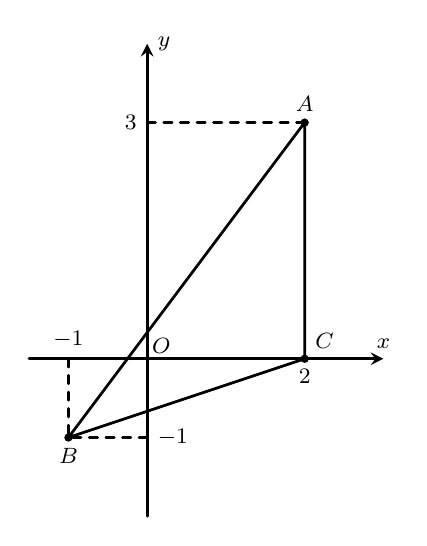
\begin{tikzpicture}[>=stealth,line join=round,line cap=round,line width=1pt,font=\footnotesize]
\draw[->](-1.5,0)--(0,0)node [above right=-2pt]{$ O $}--(3,0) node [above]{$ x $};
\draw[->](0,-2)--(0,4)node [right]{$ y $};
\coordinate[label=above:$A$](A) at (2,3);
\coordinate[label=below:$B$](B) at (-1,-1);
\coordinate[label=above right:$C$](C) at (2,0);
\foreach \toado in {(A),(B),(C)}
{
\fill \toado  circle (1.5 pt);
}
\draw (A)--(B)--(C)--(A);
\draw [dashed] (-1,0)node [above]{$ -1 $}--(B)--(0,-1)node [right]{$ -1 $};
\draw[dashed](0,3)node [left]{$ 3 $}--(A);
\node [below] at (2,0){$ 2 $};
\end{tikzpicture}
\end{center}
Gọi điểm $ C(2 ; 0) $. Suy ra, biểu thức $ T=|z-2|=MC $ (với $ M $ nằm trên đoạn $ AB$).\\
Ta có $ CA=3 $, $ CB=\sqrt{10} $.\\
Suy ra giá trị lớn nhất của biểu thức $ T $ là $ T_{max}=CM_{max}=CB=\sqrt{10}=a $ khi $ M \equiv B $.\\
Biểu thức $T$ đạt giá trị nhỏ nhất là $T_{\min } = CM_{\min }= CH$; với $H$ là hình chiếu vuông góc của điểm $C$ lên đoạn thẳng $AB$.\\
Dễ dàng tìm được đường thẳng $(AB): 4x-3y+1=0$.\\
Suy ra $ CH=d\left(C, AB \right)=\dfrac{9}{5} \Rightarrow T_{min}=CH=\dfrac{9}{5}=b$.\\
Suy ra $ a+b=\sqrt{10}+\dfrac{9}{5} $.
}
\end{ex}

\begin{ex}%[Phạm Hoàng Điệp]%[2H3K2-3]%
Trong không gian với hệ tọa độ $Oxyz$, cho điểm $H(a;b;c)$ với $a$, $b$, $c>0$. Mặt phẳng $(P)$ chứa điểm $H$ và lần lượt cắt các trục $Ox$, $Oy$, $Oz$ tại $A,B,C$ thỏa mãn $H$ là trực tâm của tam giác $ABC$. Phương trình của mặt phẳng $(P)$ là
\choice
{$\dfrac{x}{a^{2}}+\dfrac{y}{b^{2}}+\dfrac{z}{c^{2}}=\dfrac{ab+bc+ca}{abc}$}
{$\dfrac{x}{a}+\dfrac{y}{b}+\dfrac{z}{c}=3$}
{\True $ax+by+cz-a^{2}-b^{2}-c^{2}=0$}
{$a^{2}x+b^{2}y+c^{2}z-a^{3}-b^{3}-c^{3}=0$}
\loigiai{
\textbf{Cách 1}\\
Gọi $A\left(x_{0};0;0\right)$, $B\left(0 ; y_{0} ; 0\right)$, $C\left(0 ; 0 ; z_{0}\right)$.\\
Khi đó mặt phẳng $(P)$ có phương trình theo đoạn chắn là: $\dfrac{x}{x_{0}}+\dfrac{y}{y_{0}}+\dfrac{z}{z_{0}}=1$.\\
Ta có $\overrightarrow{AH}=\left(a-x_{0} ; b ; c\right)$, $\overrightarrow{BC}=\left(0 ;-y_{0} ; z_{0}\right)$, $\overrightarrow{BH}=\left(a ; b-y_{0} ; c\right)$, $\overrightarrow{AC}=\left(-x_{0} ; 0 ; z_{0}\right)$.\\
Vì $H$ là trực tâm tam giác $A B C$ nên ta có hệ\\
$ \heva{&\overrightarrow{AH} \cdot \overrightarrow{BC}=0 \\ &\overrightarrow{BH} \cdot \overrightarrow{AC}=0 \\ &H \in(ABC)&} \Leftrightarrow \heva{&-by_{0}+cz_{0}=0 \\ &-ax_{0}+cz_{0}=0 \\&\dfrac{a}{x_{0}}+\dfrac{b}{y_{0}}+\dfrac{c}{z_{0}}=1} \Leftrightarrow \heva{&y_{0}=\dfrac{c}{b}z_{0} \\ &x_{0}=\dfrac{c}{a}z_{0} \\ &\dfrac{a}{\dfrac{c}{a}z_{0}}+\dfrac{b}{\dfrac{b}{c}z_{0}}+\dfrac{c}{z_{0}}=1}\Leftrightarrow \heva{&y_{0}=\dfrac{a^{2}+b^{2}+c^{2}}{b} \\& x_{0}=\dfrac{a^{2}+b^{2}+c^{2}}{a} \\& z_{0}=\dfrac{a^{2}+b^{2}+c^{2}}{c}.}$\\
Thay vào phương trình mặt phẳng $(P)$ ta được $\dfrac{ax}{a^{2}+b^{2}+c^{2}}+\dfrac{by}{a^{2}+b^{2}+c^{2}}+\dfrac{cz}{a^{2}+b^{2}+c^{2}}=1$.\\
Hay $(P)\colon ax+by+cz-a^{2}-b^{2}-c^{2}=0.$\\
\textbf{Cách 2}\\
Ta chứng minh được $OH \perp(ABC)$ hay $OH \perp(P)$.\\
Do đó mặt phẳng $(P)$ qua $H$ và nhận $\overrightarrow{OH}(a ; b ; c)$ làm véc-tơ pháp tuyến có phương trình là \begin{center}
$a(x-a)+b(y-b)+c(z-c)=0 \Leftrightarrow ax+by+cz-a^{2}-b^{2}-c^{2}=0 .$
\end{center}
}
\end{ex}

\begin{ex}%[Thành Đức Trung, Oxyz - Tư duy mở]%[2H3K3-7]%
Trong không gian với hệ tọa độ $Oxyz$, cho mặt cầu $\left(S\right)\colon(x-1)^2 + (y-3)^2 + (z-m)^2 = 16$. Gọi $X$ là tập hợp chứa tất cả các giá trị thực của tham số $m$ để mặt cầu $\left(S\right)$ tiếp xúc với đường thẳng $d\colon\dfrac{x}{2} = \dfrac{y}{3} = \dfrac{z-1}{1}$. Tổng tất cả các phần tử của tập $X$ là
\choice
{$-\dfrac{48}{13}$}
{$\dfrac{13}{48}$}
{\True $\dfrac{48}{13}$}
{$-\dfrac{13}{48}$}
\loigiai
{
Phương trình tham số của đường thẳng $d$ là $\heva{&x=2t \\&y=3t \\&z=t+1  .}$\\
Thế vào phương trình của mặt cầu $\left(S\right)$ ta được
\[(2t-1)^2 + (3t-3)^2 + (t+1-m)^2 = 16 \Leftrightarrow 14t^2 - 2(m+10)t + m^2 - 2m -5 = 0.\]
Vì $d$ và $\left(S\right)$ tiếp xúc nhau nên phương trình trên phải có nghiệm kép, tức là
\[\Delta' = 0 \Leftrightarrow (m + 10)^2 - 14(m^2 - 2m -5) = 0\Leftrightarrow -13m^2 + 48m + 170 = 0.\]
Phương trình này có tổng hai nghiệm thực là $m_1 + m_2 = \dfrac{48}{13}$.
}
\end{ex}


\Closesolutionfile{ans}